\chapter{The QweakSimG4.cc {\em main(...)} Function}\label{CHP_III}

The {\em QweakSimG4.cc} file implements the standard {\em main()}
function for a GEANT4 simulation. As described in the GANT4 manual, an
instance of the run manager object ({\em runManager}) is created (Line
72 in Fig.~\ref{fig:MAIN1}) and initialized using the QWeak objects
(Target, Detectors, etc ...), defined in the class {\em
QweakSimDetectorConstruction}, and list of physics processes, defined
in the class {\em QweakSimPhysicsList}. The objects {\em
myQweakSimAnalysis} and {\em myQweakSimUserInformation} are
instantiated on lines 75 and 76 and are used when the run manager
object user actions are defined on lines 90 through 95. If no {\em
*.mac} input file is specified when executing the simulation then the
code between lines 103 and 114 will be executed, depending on the
setting of the environment variables regarding the user interface to
be used (see the GEANT4 installation manual). If a {\em *.mac} file is
specified as the first argument when executing the simulation then the
application is running in batch mode.  In \label{batchIII} batch mode all
commands are specified in the {\em *.mac} file.

\begin{figure}[h]
  \hspace{0cm}
  \includegraphics[scale=0.8]{./figures3/QweakSimG4-p2.eps}
  \caption{}
           \label{fig:MAIN1}
\end{figure}

\begin{figure}[h]
  \hspace{0cm}
  \includegraphics[scale=0.8]{./figures3/QweakSimG4-p3.eps}
  \caption{}
           \label{fig:MAIN2}
\end{figure}
